\section{Contrazioni}
% definizione contrazioni, pag 13.5
\begin{definition}[Contrazione]\label{def:contraz}
    Una contrazione è una funzione $f: \mathbb{N} \rightarrow \mathbb{N}$, per cui vale
    \[ f(n) < n \quad \forall n>n_0 \]
\end{definition}

\subsection{Iterate}
% definizione iterata, pag 13.6
\begin{definition}[Iterata]\label{def:iterata}
    Ad una contrazione sono associate le iterate di $f(n)$
    \[
    \begin{cases} 
        f^{(0)} (n) = n      &  i = 0 \\
        f^{(i)} (n) = f \left( f^{(i-i)} (n) \right)   &  i > 0 \\
    \end{cases}
    \]
\end{definition}
Nota: le iterate formano una successione decrescente $ f^{(0)} (n) > f^{(1)} (n) > \cdots > f^{(i)} (n) $ \\
Nella prossima sezione, l'iterata $0$ sarà associata alla radice dell'abero e all'istanza generale, l'iterata $i-esima$ rappresenterà la taglia al livello $i$ dell'albero.

\subsection{Ausiliaria}
% Def ausiliaria, pag 14.6
\begin{definition}[Ausiliaria]\label{def:ausiliaria}
    Alle iterate di una funzione si associa anche una funzione ausiliaria, che indica il maggior indice di iterata per cui il valore è ancora maggiore del valore di base. Nell'albero delle ricorrenze, questo indicherà l'ultimo livello.
    \[ f^*(n, n_0) = \max \{ i>0 : f^{(i)}(n) > n_0 \} \]
    La funzione è definita solo per $n>n_0$, per convenzione assume il valore $f^*(n,n_0)=-1$ se $ n \leq n_0$
\end{definition}

\subsection{Esempi}\label{es_iter_aus}

\subsubsection{$\bm{f(n) = n/2}$}
% pag 13.9, 14.8
Calcoliamo la forma esplicita dell'iterata e la funzione ausiliaria per
\[ f(n) = \frac{n}{2} \quad \text{con} \quad n=2^k \]
Forma esplicita iterata:
\begin{align*}
    & f^{(0)}(n) = n \\
    & f^{(1)}(n) = f(n) = \frac{n}{2} \\
    & f^{(2)}(n) = f \left( f^{(1)}(n) \right) = f \left( \frac{n}{2} \right) = \frac{n}{4} = \frac{n}{2^2} \\
    & f^{(i)}(n) = \frac{n}{2^i} 
\end{align*}
Dove la generalizzazione  è valida perché gli argomenti restano potenze di due: $n/2^i = 2^{k-i}$ \\
Calcolo funzione ausiliaria:
\begin{align*}
    & f^{(i)}(n) \mgeq n_0 
        & \text{per quali $i\:$?}\\
    & \frac{n}{2^i} \mges n_0 \\
    & 2^i \mles \frac{n}{n_0} \\
    & i < \log_2 \left( \frac{n}{n_0} \right)
        & \text{il vincolo è risolto} \\
    \rightarrow \quad & f^*(n, n_0) = \log_2 \left( \frac{n}{n_0} \right) - 1
        & \text{ne prendo il massimo} \\
    n_0 = 1 \rightarrow \quad & f^*(n, 1) = \log_2 \left( n \right) - 1
        & \text{se $n_0=1$}
\end{align*}

\subsubsection{$\bm{f(n) = n-1}$}
% pag 14, 15
Calcoliamo la forma esplicita dell'iterata e la funzione ausiliaria per
\[ f(n) = n-1 \]
Forma esplicita iterata:
\begin{align*}
    & f^{(0)}(n) = n \\
    & f^{(1)}(n) = f(n) = n-1 \\
    & f^{(2)}(n) = f \left( f^{(1)}(n) \right) = f \left( n-1 \right) = n-1-1 = n-2 \\
    & f^{(i)}(n) = n-i
\end{align*}
Calcolo funzione ausiliaria:
\begin{align*}
    & f^{(i)}(n) \mgeq n_0 
        & \text{per quali $i\:$?}\\
    & n-i \mges n_0 \\
    & i < n - n_0
        & \text{il vincolo è risolto} \\
    \rightarrow \quad & f^*(n, n_0) = n - n_0 - 1
        & \text{ne prendo il massimo} \\
    n_0 = 1 \rightarrow \quad & f^*(n, 1) = n - 2
        & \text{se $n_0=1$}
\end{align*}

\subsubsection{$\bm{f(n) = \sqrt{n}}$}
% pag 14.2, 15.2
Calcoliamo la forma esplicita dell'iterata e la funzione ausiliaria per
\[ f(n) = \sqrt{n} \quad \text{con} \quad n=2^{2^k} \]
Forma esplicita iterata:
\begin{align*}
    & f^{(0)}(n) = n \\
    & f^{(1)}(n) = f(n) = \sqrt{n} = n^{\nicefrac{1}{2}} \\
    & f^{(2)}(n) = f \left( f^{(1)}(n) \right) = f \left( n^{\nicefrac{1}{2}} \right) = n^{\nicefrac{1}{2^2}} \\
    & f^{(i)}(n) = n^{\nicefrac{1}{2^i}} \\
\end{align*}
Calcolo funzione ausiliaria:
\begin{align*}
    & f^{(i)}(n) \mgeq n_0 
        & \text{per quali $i\:$?}\\
    & n^{\nicefrac{1}{2^i}} \mges n_0 \\
    & \log_2 n^{\nicefrac{1}{2^i}} \mges \log_2 n_0 \\
    & \frac{1}{2^i} \log_2 n \mges \log_2 n_0 \\
    & 2^i \mles \frac{\log_2 n}{\log_2 n_0} \\
    & i < \log_2 \frac{\log_2 n}{\log_2 n_0} 
        & \text{il vincolo è risolto} \\
    & i < \log_2 \log_2 n + \log_2 \log_2 n_0 \\
    \rightarrow \quad & f^*(n, n_0) = \log_2 \log_2 n + \log_2 \log_2 n_0 - 1
        & \text{ne prendo il massimo} \\
    n_0 = 2 \rightarrow \quad & f^*(n, 2) = \log_2 \log_2 n - 1
        & \text{se $n_0=2$}
\end{align*}
Il vincolo su $n$ può essere generalizzato a $n=a^{2^k}$, in questo caso $n_0 = a$

\subsubsection{$\bm{f(n) = \left\lfloor n/2 \right\rfloor}$}
Nel caso $f(n) = \left\lfloor n/2 \right\rfloor$, si può dimostrare che
$ f^{(2)}(n) = \left\lfloor \left\lfloor n/2 \right\rfloor / 2 \right\rfloor = \left\lfloor n / 2^2 \right\rfloor $
ma non è per niente banale.

\section
[Modifica al \textit{Divide and Conquer}]
{Modifica al \textit{Divide and Conquer} \\ 
{ \large Risoluzione di una classe generale di ricorrenze\\ associate ad algoritmi \textit{Divide and Conquer} } }
% titolo meno informativo della storia
% sottotitolo già meglio
\subsection{Meta-algoritmo}
% Metaalgoritmo DnC modificato, pag 12.5
\begin{algorithm}[H]
\caption{Divide and Conquer modificato}\label{alg:dncm}
\begin{algorithmic}[1]
    \Procedure{D\&C}{$i$}
        \State $n=|i|$
        \If{$n \leq n_0$}                             \Comment{BASE}
            \State *risolvo direttamente*
        \EndIf
        \State $<i_1, i_2, \dots, i_{S(n)}> \gets A_D(i)$    \Comment{DIVIDE}
        \For{$j \gets 1 $ to $ {S(n)} $ }                    \Comment{RECURSE}
            \State $s_j \gets $ \Call{D\&C}{$i_j$}
        \EndFor
        \State $s \gets A_C(<s_1, s_2, \dots, s_{S(n)}>)$    \Comment{CONQUER}
        \State return $s$
    \EndProcedure
\end{algorithmic}
\end{algorithm}
% Parametri noti, pag 13
L'algoritmo ha dei vincoli in più rispetto al prototipo generico, in particolare sul numero e dimensione delle sottoistanze generate. I parametri che lo descrivono sono:
\begin{itemize}[noitemsep,topsep=0pt,parsep=0pt,partopsep=0pt]
    \item[--] $S(n): \mathbb{N} \rightarrow \mathbb{N}$ \\
        istanze di taglia $n$ nella fase di \textit{Divide} generano sempre lo \textbf{stesso} numero di sottoistanze
    \item[--] $ |i_j| = f(n) < n \quad \forall j : 1 \leq j \leq S(n) $ \\
        le sottoistanze sono sempre grandi uguali
    \item[--] $ w(n) = T_{A_D}(n) + T_{A_C}(n)$ \\
        lavoro compiuto per ogni istanza per dividere e ricomporre
    \item[--] $n_0$ taglia del caso base
    \item[--] $T_0$ tempo al caso peggiore di risoluzione diretta quando $|i| \leq n_0$
\end{itemize}
% Nuova eq di ricorrenza, pag 13.3
L'equazione di ricorrenza diventa
\[
    T(n) = 
    \begin{cases} 
        T_0      &  n \leq n_0 \\
        S(n) \, T(f(n)) + w(n) & n > n_0
    \end{cases}
\]
Ad ogni passo vengono fatte $S(n)$ chiamate ricorsive su istanze grandi $f(n)$

\subsubsection{esempio parametri MAX}
% parametri max, pag 13.5
I parametri del $MAX$ sono, con la nuova notazione:\\
$S(n)=2$, $f(n)=n/2$, $w(n)=1$, $T_0=0$, $n_0=1$

\subsection{Equazione delle ricorrenze generica}
% Alberone, pag 15.8
% { \centering
\begin{center}
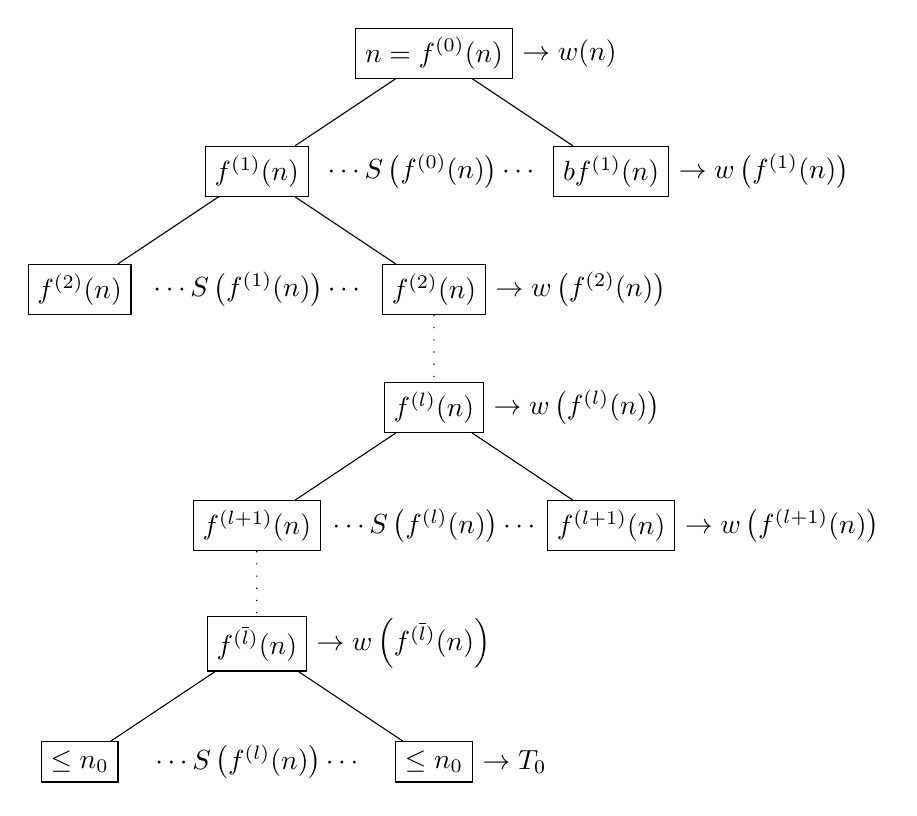
\begin{tikzpicture}[
  level/.style={sibling distance=45mm},
  every node/.style={rectangle,draw,solid},
  dotme/.style={edge from parent/.style={loosely dotted,draw}},
  norm/.style={edge from parent/.style={solid,draw}}
  ]
  \node [label=right:{$\rightarrow w(n)$}] (z){$n = f^{(0)}(n)$}
    child { node (a) {$f^{(1)}(n)$}
      child { node (c) {$f^{(2)}(n)$}
      }
      child { node [label=right:{$\rightarrow w\left(f^{(2)}(n)\right)$}] (d) {$f^{(2)}(n)$}
        child [dotme] { node [label=right:{$\rightarrow w\left(f^{(l)}(n)\right)$}] 
                (d1) {$f^{(l)}(n)$}
          child [norm] { node (e) {$f^{(l+1)}(n)$}
            child [dotme] { node [label=right:{$\rightarrow
                            % w\left(f^{\left(\overline{l}\right)}(n)\right)$}] 
                            % nessuno dei due è decente
                            w\left(f^{(\overline{l})}(n)\right)$}]
                            (e1) {$f^{(\overline{l})}(n)$}
              child [norm] { node (g) {$\leq n_0$}
              }
              child [norm]{node[label=right:{$\rightarrow T_0$}]
                       (h) {$\leq n_0$}
              }
            }
          }
          child [norm] { node [label=right:{$\rightarrow w\left(f^{(l+1)}(n)\right)$}]
                   (f) {$f^{(l+1)}(n)$}
          }
        }
      }
    }
    child { node [label=right:{$\rightarrow w\left(f^{(1)}(n)\right)$}] (b) {$b f^{(1)}(n)$}
    }
  ; % end of the node
  \path (a) -- (b) node [draw=none,midway] {$\cdots S\left(f^{(0)}(n)\right) \cdots$ };
  \path (c) -- (d) node [draw=none,midway] {$\cdots S\left(f^{(1)}(n)\right) \cdots$ };
  \path (e) -- (f) node [draw=none,midway] {$\cdots S\left(f^{(l)}(n)\right) \cdots$ };
  \path (g) -- (h) node [draw=none,midway] {$\cdots S\left(f^{(l)}(n)\right) \cdots$ };
  % \draw (e) -- (f) node [draw=none,midway,loosely dotted,above=10pt] {$S(f^{(l)}(n)) $ };
\end{tikzpicture}
\end{center}
% } % end centering, LASCIA la riga sopra questa parentesi (serve un \par)
% \usetikzlibrary{positioning}
% \node[nome,right] (p2) [below = of p1] {text text};

Nell'albero la taglia delle istanze è indicata nel nodo, il lavoro associato (uguale per ogni istanza del livello) è indicato a fianco del livello. Il numero di sottoistanze generate da ciascuna istanza di un livello è indicato tra i nodi figli. Si indica con $l \leq f^*(n,n_0)$ un generico livello interno e con $\overline{l} = f^*(n,n_0)$ l'ultimo livello interno. I nodi foglia sono tutti di dimensione minore del caso base, ed è a loro associato il lavoro $T_0$ necessario a risolverli direttamente.

Da questo albero delle ricorrenze si può ricavare il lavoro totale, sommando i contributi di ciascun nodo.
% Formulone, pag 16
% \begin{align*}
    % T(n) & = \sum_{l=0}^{f^*(n,n_0)}\text{\# nodi nel livello}\cdot\text{\# $w$ per nodo del livello}+\text{contributo foglie}\\
    % &= \sum_{l=0}^{f^*(n,n_0)} \left[ \prod_{j=0}^{l-1} S \left( f^{(j)}(n) \right) \cdot w \left( f^{(l)}(n) \right) \right] +
        % \prod_{j=0}^{f^*(n,n_0)} S \left( f^{(j)}(n) \right) \cdot T_0
% \end{align*}
\begin{equation}
    \begin{aligned}[b]
    T(n) & = \sum_{l=0}^{f^*(n,n_0)}\text{\# nodi nel livello}\cdot\text{\# $w$ per nodo del livello}+\text{contributo foglie}\\
    &= \sum_{l=0}^{f^*(n,n_0)} \left[ \prod_{j=0}^{l-1} S \left( f^{(j)}(n) \right) \cdot w \left( f^{(l)}(n) \right) \right] +
        \prod_{j=0}^{f^*(n,n_0)} S \left( f^{(j)}(n) \right) \cdot T_0
        \label{eq:formachiusaric}
    \end{aligned}
\end{equation}


Da qualche parte le convenzioni sugli operatori, pag 15.5; insieme alle cose a fine capitolo DnC -$>$ Appendice

\subsubsection{Esempio formula}
% Esempio, pag 16.5
Risolviamo l'equazione di ricorrenza utilzzando la formula appena ottenuta.
\[
    T(n) = 
    \begin{cases} 
        4      &  n = 1 \\
        6 \, T\left(\frac{n}{3}\right) + n^2-n & n > 1 \quad \text{assumendo } n=3^k
    \end{cases}
\]
Da cui ricaviamo i valori dei parametri:
\begin{align*}
    S(n)&=6 & f(n)&=\frac{n}{3} & w(n)&=n^2-n & T_0&=4 & n_0&=1
\end{align*}
Le formule di iterata $i-esima$ e ausiliaria si ricavano come spiegato nella sezione \ref{es_iter_aus}:
\begin{align*}
    f^{(i)}(n) &= \frac{n}{3^i} & f^*(n, 1) &= \log_3 \left( n \right) - 1
\end{align*}
Calcoliamo le componenti interne della formula:
% \begin{gather*}
\begin{align*}
    \prod_{j=0}^{l-1} S \left( f^{(j)}(n) \right) 
    &= \prod_{j=0}^{l-1} 6 = 6^{l-1+1} = 6^l \\
    w\left(f^{(l)}(n) \right) 
    &=  w \left( \frac{n}{3^l} \right) 
    = \frac{n^2}{3^{2l}} - \frac{n}{3^l} = \frac{n^2}{9^l}-\frac{n}{3^l} \\
    \prod_{j=0}^{f^*(n,n_0)} S \left( f^{(j)}(n) \right) 
    &= \prod_{j=0}^{\log_3 n-1} 6 = 6^{\log_3 n} =
    n^{\log_3 6} = n^{\log_3 (2\cdot3)} = n^{\log_3 2 + \log_3 3} = n^{\log_3 2 + 1}
% \end{gather*}
\end{align*}
La formula risulta quindi:
\begin{align*}
    T(n) & = \sum_{l=0}^{\log_3 n-1} 6^l \left( \frac{n^2}{9^l}-\frac{n}{3^l} \right) + 4 n^{\log_3 2 + 1} \\
    & = n^2\,\sum_{l=0}^{\log_3 n-1} \left( \frac{2}{3} \right)^l - n\,\sum_{l=0}^{\log_3 n-1} 2^l+ 4 n^{\log_3 2+1} \\
    & = n^2 \left( \frac{1- \left( 2/3 \right)^{\log_3 n} }{1 - 2/3 } \right) - n(2^{\log_3 n} -1) + 4 n^{\log_3 2+1} 
    % & \left[ \left( \frac{2}{3} \right)^{\log_3 n} &= \frac{2^{\log_3 n}}{3^{\log_3 n}} = \frac{n^{\log_3 2}}{n}\right]\\
    &
    \left[
    \left( \frac{2}{3} \right)^{\log_3 n}
    \right. % tutto questo per avere le parentesi quadre grandi
    &=      % attorno a sto maledetto align
    \left.  % che avrei anche potuto spostare 
    \frac{2^{\log_3 n}}{3^{\log_3 n}} = \frac{n^{\log_3 2}}{n}
    \vphantom{\left( \frac{2}{3} \right)^{\log_3 n}}
    \right] % ma grandi quanto voglio io
    \\
    & = 3n^2 \left( 1- \frac{n^{\log_3 2}}{n} \right) - n \left( n^{\log_3 2}-1 \right) + 4 n^{\log_3 2+1} \\
    & = 3n^2 -3n^{1+\log_3 2} - n^{1+\log_3 2} + n + 4 n^{1+\log_3 2} \\
    & = 3n^2+n
\end{align*}
È una buona idea verificare la correttezza per induzione:\\
Base: 
\[ T(1)=4 \meq \left( 3n^2+n \right) \Big|_{n=1} = 4 \rightarrow \text{vera} \]
Ipotesi: Considero corretta la formula per i valori $s<n$ nella forma $s=3^k$ \\
Tesi:
\begin{align*}
    T(n) &= 6T \left( \frac{n}{3} \right) + n^2 -n \\
    & = 6 \left( 3 \frac{n^2}{9} + \frac{n}{3} \right) \\
    & = 3n^2+n\rightarrow \text{vera}
\end{align*}

\subsubsection{Esempio formula}
% Esempio, pag 17.5
\[
    T(n) = 
    \begin{cases} 
        1      &  n = 2 \\
        2 \, T\left( \sqrt{n}\right) + 1 & n > 2 \quad \text{assumendo } n=2^{2^k} 
    \end{cases}
\]
Le formule di iterata $i-esima$ e ausiliaria si ricavano come spiegato nella sezione \ref{es_iter_aus}:
\begin{align*}
    T(n) &= \sum_{l=0}^{\log_2 \log_2 n-1} 2^l \cdot 1 + 2^{\log_2 \log_2 n} \cdot 1 \\
    &= 2^{\log_2 \log_2 n} -1 + 2^{\log_2 \log_2 n} 
    && \left[ 2^{\log_2 \log_2 n} = \log_2 n ^{\cancel{\log_2 2}} \right] \\
    &= 2 \log_2 n - 1
\end{align*}

\section{\textit{Master Theorem}}
\subsection{Ipotesi}
% Ipotesi, pag 18
Il \textit{Master Theorem} è valido per sottoclassi di ricorrenze in cui:
\begin{enumerate}
    \item $S(n) = a$ con $a$ costante, $a \geq 1$ (almeno un'istanza viene generata)
    \item $f(n) = \frac{n}{b}$ con $b$ costante, $b > 1$ (deve essere una contrazione)
    \item $w(n): \mathbb{N}^+ \rightarrow \mathbb{N}^+$% \setminus \{0\}$ % ???
    \item $T_0 > 1$ ($ T_0 = 0$ è ragionevole ma non vale la dimostrazione)
    \item $n_0 \in \mathbb{N}$
\end{enumerate}
La formula di ricorrenza è quindi nella forma:
\begin{equation}
    T(n) = 
    \begin{cases} 
        T_0      &  n \leq n_0 \\
        a \, T\left( \frac{n}{b} \right) + w(n) & n > n_0 \quad \text{assumendo } n=b^k
    \end{cases}
    \label{eq:masterricorrenza1}
\end{equation}

\subsection{Tesi}
% Tesi, pag 18.5
% \[
% T(n) = 
% % \begin{numcases}
% \begin{cases}
    % \Theta (n^{\log_b a}) & \text{se } \exists \varepsilon > 0 : w(n) = O(n^{\log_b a-\varepsilon})\\
    % \Theta (n^{\log_b a} \, \log_n) & \text{se } w(n) = \Theta(n^{\log_b a})\\
    % \Theta (w(n)) & \text{se }
    % \begin{cases}
    % % \begin{numcases}
        % \exists \varepsilon > 0 : w(n) = \Omega(n^{\log_b a+\varepsilon})\\
        % \exists 0<c<1 : \forall n \in \mathbb{N}-\{0\} : a w \left( \frac{n}{b} \right) < c w(n)
    % % \end{numcases}
    % \end{cases}
% % \end{numcases}
% \end{cases}
% \]

% \begin{numcases}{T(n)=}
    % \Theta (n^{\log_b a}) & se $\exists \varepsilon > 0 : w(n) = O(n^{\log_b a-\varepsilon})$\\
    % \Theta (n^{\log_b a} \, \log_n) & se $w(n) = \Theta(n^{\log_b a})$\\
    % \Theta (w(n)) & condition
    % % \begin{subnumcases}{se}
        % % \exists \varepsilon > 0 : w(n) = \Omega(n^{\log_b a+\varepsilon})\\
        % % \exists 0<c<1 : \forall n \in \mathbb{N}-\{0\} : a w \left( \frac{n}{b} \right) < c w(n)
    % % \end{subnumcases}
% \end{numcases}
% \textbf{Caso 1:} 
% \begin{equation}
    % T(n) = \Theta (n^{\log_b a})  \text{ se } \exists \varepsilon > 0 : w(n) = O(n^{\log_b a-\varepsilon})
    % \label{eq:mastercaso1}
% \end{equation}

Ci sono tre casi possibili:\\
\begin{description}
    \item[\textbf{Caso 1:}] 
        \begin{equation}
            T(n) = \Theta (n^{\log_b a})  \text{ se } \exists \varepsilon > 0 : w(n) = O(n^{\log_b a-\varepsilon})
            \label{eq:mastercaso1}
        \end{equation}
    \item[\textbf{Caso 2:}] 
        \begin{equation}
            T(n) = \Theta (n^{\log_b a} \, \log_n) \text{ se } w(n) = \Theta(n^{\log_b a})
            \label{eq:mastercaso2}
        \end{equation}
    \item[\textbf{Caso 3:}] 
        \begin{subnumcases}{T(n) = \Theta (w(n)) \text{ se }}
            \exists \varepsilon > 0 : w(n) = \Omega(n^{\log_b a+\varepsilon})
            \label{eq:mastercaso3a}\\
            \exists 0<c<1 : \forall n \in \mathbb{N} \setminus \{0\} : a w \left( \frac{n}{b} \right) < c w(n)
            \label{eq:mastercaso3b}
        \end{subnumcases}
\end{description}

Note:
\begin{itemize}
    \item[--] $n^{\log_b a}$ è detta funzione di soglia, o \textit{threshold}
    \item[--] la condizione \ref{eq:mastercaso3b} è detta condizione di regolarità, indica che $w(n)$ è non decrescente, e quando cresce lo fa in modo uniforme
\end{itemize}

\subsection{Dimostrazione}
\subsubsection{Considerazioni sui parametri}
% Considerazioni sull'asintotico, pag 18.9, 19
Il parametro $n_0$, con $T_0>0$, rende alcuni passaggi della dimostrazione più difficili. Lo si può assumere come il primo elemento della famiglia $b^k=b^0=1$? Considerando i nodi foglia dell'albero delle ricorrenze, hanno tutti taglia $n_0$ e lavoro associato $T_0$. Continuando a dividere i nodi finché raggiungono taglia $1$, si generano dei sotto-alberi alti $\log_b \left( n_0 \right)$, con nodi foglia di taglia $1$, a ciascuno dei quali è associato ancora il lavoro $T_0$, essendo il lavoro al caso peggiore. Il lavoro associato ai sotto-alberi è quindi $O(1)$ (costante), e senza perdita di generalità si può considerare $n_0=1$.

\subsubsection{Considerazioni sulle relazioni asintotiche}
% Considerazioni sull'asintotico, pag 18.9, 19
Per funzioni intere positive $g: \mathbb{N} \setminus \{0\} \rightarrow  \mathbb{N} \setminus \{0\}$, si può modificare la definizione delle maggiorazioni e minorazioni asintotiche.
\begin{description}
    \item[$\bm{T(n)=O \left( g(n) \right)}$:]
        $T$ è \textit{O-grande} di $g$ ($T$ è asintoticamente minore di $g$) se vale
        $$T(n) = O\left(g(n)\right)\text{ se }\exists c>0,\overline{n}:
            \forall n>\overline{n}\Rightarrow T(n)\leq c\cdot g(n) \qquad \circola{A}$$
        mostriamo che per le funzioni intere positive, $\overline{n}=1$
        $$T(n) = O\left(g(n)\right)\text{ se }\exists c'>0:
            \forall n>1 \Rightarrow T(n)\leq c'\cdot g(n) \qquad \circola{B}$$
        dimostriamo $ \circola{A} \Rightarrow \circola{B}$
        $$ \text{sia } \overline{c} = \max \left\{ c, T(1), T(2), \dots, T( \overline{n} ) \right\} $$
        verifico che $ \forall n>1 \rightarrow T(n) \leq \overline{c} g(n) $
        \begin{itemize}[noitemsep,topsep=0pt,parsep=0pt,partopsep=0pt]
            \item $1 \leq n \leq \overline{n} \rightarrow T(n) \leq \overline{c} \leq \overline{c}g(n) $ \\
                la prima valida per definizione di $ \overline{c} $, la seconda perché $g$ è intera positiva
            \item $ n > \overline{n} \rightarrow T(n) \leq cg(n) \leq \overline{c}g(n)$ \\
                la prima valida perché $T=O(G)$, la seconda per definizione di $\overline{c}$
        \end{itemize}
    \item[$\bm{T(n)=\Omega \left( g(n) \right)}$:]
        $T$ è \textit{omega} di $g$ ($T$ è asintoticamente maggiore di $g$) se vale
        $$T(n) = \Omega \left(g(n)\right)\text{ se }\exists c>0,\overline{n}:
            \forall n>\overline{n}\Rightarrow T(n)\geq c\cdot g(n) \qquad \circola{A}$$
        mostriamo che per le funzioni intere positive, $\overline{n}=1$
        $$T(n) = \Omega \left(g(n)\right)\text{ se }\exists c'>0:
            \forall n>1 \Rightarrow T(n)\geq c'\cdot g(n) \qquad \circola{B}$$
        dimostriamo $ \circola{A} \Rightarrow \circola{B}$
        $$ \text{sia } \overline{c} = \min \left\{ c, \frac{T(1)}{g(1)}, \frac{T(2)}{g(2)} ,
            \dots, \frac{T( \overline{n})}{ g( \overline{n}) } \right\} $$
        verifico che $ \forall n>1 \rightarrow T(n) \geq \overline{c} g(n) $
        \begin{itemize}[noitemsep,topsep=0pt,parsep=0pt,partopsep=0pt]
            \item $1 \leq n \leq \overline{n} \rightarrow T(n) = \frac{T(n)}{g(n)}g(n) \geq \overline{c}g(n) $ \\
                per definizione di $ \overline{c} $ come minimo dei valori
            \item $ n > \overline{n} \rightarrow T(n) \geq cg(n) \geq \overline{c}g(n)$ \\
                la prima valida perché $T=\Omega(G)$, la seconda per definizione di $\overline{c}$
        \end{itemize}
    \item[$\bm{T(n)=\Theta \left( g(n) \right)}$:] $T=\Omega(G)$ e $T=O(g)$ implicano $T=\Theta(g)$
\end{description}

\subsubsection{Costo delle foglie}
Ricordiamo che 
\begin{align*}
    f(n)&= \frac{n}{b} & f^{(j)}(n) &= \frac{n}{b^j} & f^*(n,1) &= \log_b n -1
\end{align*}

Per cui la formula risulta:
\begin{equation}
    \begin{aligned}[b]
        T(n) &= \sum_{l=0}^{\log_b n -1} \left[ a^l \cdot w \left( \frac{n}{b^l} \right) \right] + a^{\log_b n} \cdot T_0 \\
        &= \sum_{l=0}^{\log_b n -1} \left[ a^l \cdot w \left( \frac{n}{b^l} \right) \right] + n^{\log_b a} \cdot T_0
        \label{eq:masterchiusa1}
    \end{aligned}
\end{equation}

In cui possiamo notare la presenza della funzione di soglia come numero di foglie dell'albero. In più, avendo imposto (per ora) $T_0>0$, è triviale dedurre \begin{equation}
    n^{\log_b a} \cdot T_0 = \Theta \left( n^{\log_b a} \right) 
    \label{eq:masterfoglie}
\end{equation}

% \subsubsection{Dimostrazione caso 1}
\subsubsection{Caso 1}
% Dimostrazione, pag 20
% Vogliamo dimostrare il caso $1$:
Dimostriamo ora il caso $1$, di cui riportiamo l'enunciato:
    \begin{align*}
        \exists \varepsilon > 0 &: w(n) = O(n^{\log_b a-\varepsilon})
        \Rightarrow
        T(n) = \Theta \left( n^{\log_b a} \right) 
    \end{align*}
\begin{proof}
    \begin{align*}
        \intertext{Per ipotesi}
        \exists \varepsilon > 0 , \exists c>0 &: \forall n>1 \rightarrow w(n) \leq cn^{\log_b a-\varepsilon} \\
        \intertext{maggioriamo il primo termine della formula \ref{eq:masterchiusa1}, ricavandone il limite superiore asintotico cercato:}
        \sum_{l=0}^{\log_b n -1} a^l \cdot w \left( \frac{n}{b^l} \right)
        & \leq c \sum_{l=0}^{\log_b n -1} a^l \cdot \left( \frac{n}{b^l} \right)^{\log_b a - \varepsilon} 
        & w=O \left( n^{\log_b a - \varepsilon} \right) & \\
        & = c n^{\log_b a - \varepsilon} \sum_{l=0}^{\log_b n -1} \frac{a^l}{b^{l^{\log_b a}} b^{l^{-\varepsilon}}}
        & b^{l^{\log_b a}} = b^{\log_b a^{l}} = a^l & \\
        & = c n^{\log_b a - \varepsilon} \sum_{l=0}^{\log_b n -1} \frac{\cancel{a^l}}{\cancel{a^l} b^{-\varepsilon^l}} \\
        & = c n^{\log_b a - \varepsilon} \sum_{l=0}^{\log_b n -1} b^{\varepsilon^l}
        & \text{se } b>1, \, b^{\varepsilon}>1 & \\
        & = c n^{\log_b a - \varepsilon} \left( \frac{b^{\varepsilon^{\log_b n}} - 1}{b^{\varepsilon} - 1} \right) \\
        & = c n^{\log_b a - \varepsilon} \left( \frac{n^{\varepsilon} - 1}{b^{\varepsilon} - 1} \right) \\
        & \leq c n^{\log_b a - \varepsilon} \left( \frac{n^{\varepsilon} }{b^{\varepsilon} - 1} \right) \\
        & \leq c\frac{ n^{\log_b a - \varepsilon + \varepsilon} }{b^{\varepsilon} - 1} \\
        & \leq \frac{ c }{b^{\varepsilon} - 1} n^{\log_b a}
        & c, b, \varepsilon \text{ sono costanti} &\\
        % \intertext{quindi la sommatoria è $O-grande$ di $n^{\log_b a}$}
        % \sum_{l=0}^{\log_b n -1} a^l \cdot w \left( \frac{n}{b^l} \right)
        & = O \left( n^{\log_b a} \right)
        \intertext{combinando questo risultato con \ref{eq:masterfoglie} si ottiene}
        T(n) & = O \left( n^{\log_b a} \right) + \Theta \left( n^{\log_b a} \right) 
        \intertext{per le leggi sui vincoli asintotici, $O$ è implicato da $\Theta$}
        T(n) & = \Theta \left( n^{\log_b a} \right) 
    \end{align*}
\end{proof}
Nel caso 1 la maggior parte del lavoro è svolto dai nodi foglia.\\
Nota: se $T_0=0$, \ref{eq:masterfoglie} non è valida, e risulta nullo il contributo delle foglie: 
$T(n) = O \left( n^{\log_b a} \right) $

\subsubsection{Caso 2}
% Dimostrazione, pag 21
% Vogliamo dimostrare il caso $2$:
Dimostriamo ora il caso $2$, di cui riportiamo l'enunciato:
    \begin{align*}
        w(n) = \Theta(n^{\log_b a})
        & \Rightarrow
        T(n) = \Theta \left( n^{\log_b a} \log n \right) 
    \end{align*}
\begin{proof}
    \begin{align*}
        \intertext{Per ipotesi}
        \exists c_1, c_2 : \forall n \geq 1 & \rightarrow c_1 n^{\log_b a} \leq w(n) \leq n^{\log_b a}
        \intertext{usiamo la seconda disequazione per maggiorare la sommatoria}
        \sum_{l=0}^{\log_b n -1} a^l \cdot w \left( \frac{n}{b^l} \right)
        & \leq c_2 \sum_{l=0}^{\log_b n -1} a^l \left( \frac{n}{b^l} \right)^{\log_b a} \\
    % & = c_2 \sum_{l=0}^{\log_b n -1} \frac{\cancel{a^l}}{\cancel{a^l}} n^{log_b a}
        & = c_2 \sum_{l=0}^{\log_b n -1} \frac{a^l n^{\log_b a}}{a^l} 
        & b^{l^{\log_b a}} = a^l &\\
        & = c_2 n^{\log_b a} \sum_{l=0}^{\log_b n -1} 1 \\
        & = c_2 n^{\log_b a} \log_b n \\
        % \intertext{quindi la sommatoria è $O-grande$ di $n^{\log_b a} \log n$}
        % \sum_{l=0}^{\log_b n -1} a^l \cdot w \left( \frac{n}{b^l} \right)
        & = O \left( n^{\log_b a} \log n \right) \\
        \intertext{in modo analogo la si minora con $c_1$}
        \sum_{l=0}^{\log_b n -1} a^l \cdot w \left( \frac{n}{b^l} \right)
        & \geq c_1 \sum_{l=0}^{\log_b n -1} a^l \left( \frac{n}{b^l} \right)^{\log_b a} \\
        & = c_1 n^{\log_b a} \log_b n \\
        % \intertext{quindi la sommatoria è $\Omega-grande$ di $n^{\log_b a} \log n$}
        % \sum_{l=0}^{\log_b n -1} a^l \cdot w \left( \frac{n}{b^l} \right)
        & = \Omega \left( n^{\log_b a} \log n \right) \\
        \intertext{combinando i due risultati}
        \sum_{l=0}^{\log_b n -1} a^l \cdot w \left( \frac{n}{b^l} \right)
        & = \Theta \left( n^{\log_b a} \log n \right) \\
        \intertext{combinando questo risultato con \ref{eq:masterfoglie} si ottiene}
        T(n) & = \Theta \left( n^{\log_b a} \right) + \Theta \left( n^{\log_b a} \log n \right) \\
        \intertext{per le leggi sui vincoli asintotici, il primo contributo è trascurabile}
        T(n) & = \Theta \left( n^{\log_b a} \log n \right) \\
    \end{align*}
\end{proof}
In questo caso la maggior parte del lavoro è compiuta all'interno dell'albero, ogni livello compie lo stesso lavoro cumulativo, e ci sono $\log n$ livelli. L'esempio principale del caso 2 è il \textit{Merge-Sort}, descritto da $T(n)=2T(n/2)+n$, dove ogni livello compie $n^{\log_2 2}=n$ operazioni e la complessità è $\Theta (n \log n)$.

\subsubsection{Caso 3}
% Dimostrazione, pag 22
Prima di dimostrare il caso 3, dimostriamo il seguente lemma sulla condizione di regolarità estesa
\begin{lemma}
    Se una funzione è regolare $\left( \exists c, 0 \leq c \leq 1 : \forall n \rightarrow aw\left( \frac{n}{b} \right) \leq cw(n) \right) $
    vale \[ \forall l \geq 1 \quad a^l w\left( \frac{n}{b^l} \right) \leq c^l w(n) \]
    \label{teo:regestesa}
\end{lemma}
\begin{proof}
    Dimostriamo il lemma per induzione. La base, per $l=1$, coincide con l'ipotesi di regolarità. Ipotizzando il lemma sia valido per $l'<l$, dimostriamo che vale per $l$.
    \begin{align*}
        a^l w\left( \frac{n}{b^l} \right)
        &= a^{l-1} a w \left( \frac{n/b^{l-1}}{b} \right)
        & \text{per la regolarità } a w \left( \frac{n/b^{l-1}}{b} \right) \leq cw \left( \frac{n}{b^{l-1}} \right)&\\
        & \leq a^{l-1} cw \left( \frac{n}{b^{l-1}} \right)
        & \text{per l'HP induttiva } a^{l-1} \left( \frac{n}{b^{l-1}} \right) \leq c^{l-1}w(n)&\\
        & \leq cc^{l-1}w(n) \\
        & = c^lw\left( n \right)
    \end{align*}
\end{proof}
Dimostriamo ora il caso $3$, di cui riportiamo l'enunciato:
    \begin{align*}
        a) \quad &\exists \varepsilon > 0 : w(n) = \Omega(n^{\log_b a+\varepsilon}) \\
        b) \quad &\exists c, 0 \leq c \leq 1 : \forall n \rightarrow aw\left( \frac{n}{b} \right) \leq cw(n) \\
        \Rightarrow \quad & T(n) = \Theta \left( w(n) \right)
    \end{align*}
\begin{proof}
\begin{align*}
    \sum_{l=0}^{\log_b n -1} a^l \cdot w \left( \frac{n}{b^l} \right)
    & \leq \sum_{l=0}^{\log_b n -1} c^l \cdot w(n) \\
    & \leq w(n) \sum_{l=0}^{+\infty} c^l & c<1 &\\
    & = \frac{1}{1-c}w(n) \\
    % \intertext{quindi la sommatoria è $O-grande$ di $w(n)$}
    % \sum_{l=0}^{\log_b n -1} a^l \cdot w \left( \frac{n}{b^l} \right)
    & = O \left (w(n) \right) \\
    \intertext{combinando questo risultato con \ref{eq:masterfoglie} si ottiene}
    T(n) & = \Theta \left( n^{\log_b a} \right) + O\left( w(n) \right)
    \intertext{per le leggi sui vincoli asintotici, il primo contributo è trascurabile}
    T(n) & = O\left( w(n) \right)
    \intertext{per $n>1$ osserviamo}
    T(n) &= aT\left( \frac{n}{b} \right) w(n) \geq w(n)
    & \text{$a$ e $T$ positive} &\\
    T(n) & = \Omega \left( w(n) \right) 
    \intertext{da cui ricaviamo}
    T(n) & = \Theta \left( w(n) \right)
\end{align*}
\end{proof}

\subsection{Accortezze sulle ipotesi}
% esempio ipotesi non rispettate, pag 22.9, 23
Quando si applica la formula, si deve fare attenzione durante la verifica delle ipotesi.
Il fatto che una funzione $w(n)$ non sia $O(n)$ e neppure $\Theta(n)$ \textit{non} implica che essa sia $\Omega(n)$. Per esempio
\[
    T(n) = 
    \begin{cases} 
        1      &  n = 1 \\
        2 \, T\left(\frac{n}{2}\right) + n \log_2 n & n > 1 \quad \text{assumendo } n=2^k
    \end{cases}
\]
ha come \textit{threshold} $n^{\log_b a} = n$ per cui
\begin{description}
    \item[Caso 1:] $w(n) \meq O(n) \rightarrow $ no, è strettamente maggiore
    \item[Caso 2:] $w(n) \meq \Theta(n) \rightarrow $ no, è un infinito di ordine superiore
    \item[Caso 3:] $w(n) \meq \Omega(n) \rightarrow $
        no! $w(n)$ deve essere \textit{polinomialmente} più grande, e non è così
        \begin{align*}
            \exists \, \varepsilon > 0 :\, & w(n) = \Omega \left( n^{1+\varepsilon} \right) \\
            & n \log_n n = \Omega \left( n^{1+\varepsilon} \right) \\
            & \log_n n = \Omega \left( n^{\varepsilon} \right) \rightarrow
                \text{ mai verificato per nessun $\varepsilon$}
        \end{align*}
        il \textit{Master Theorem} nel caso tre sosterrebbe $T(n)=\Omega \left( n \log_n n \right)$
        commettendo un errore. Applicando la formula \ref{eq:formachiusaric}, le cui ipotesi sono invece tutte rispettate, otteniamo infatti
        \begin{align*}
            T(n) &= \sum_{l=0}^{\log_2 n} 2^l \left( \frac{n}{2^l} \log_2 \left( \frac{n}{2^l} \right) \right) + 2^{\log_2 n} \cdot 1 \\
            & \left[ \log_2 \left( \frac{n}{2^l} \right) + 2^{\log_2 n} = \log_2 n - \log_2 2^l = \log_2 n - l \log_2 2 \right] \\
            & = n + n \sum_{l=0}^{\log_2 n} \left( \log_2 n - l \right) \\
            & \left[ \text{cambio di variabile } k = \log_2n-l \quad
                l=0 \rightarrow k=\log_2 n \quad l=\log_2 n -1 \rightarrow k=1 \right] \\
            & = n + n \sum_{l=0}^{\log_2 n} k \\
            & = n + n \frac{\left( \log_2 n \right) \left( \log_2 n + 1 \right)}{2} \\
            & = n + \frac{n \log_2^2 n }{2}  + \frac{n \log_2 n }{2} \\
            & = \Theta \left( n \log_2^2 n \right) 
        \end{align*}
\end{description}

\subsection{Regolarità dei polinomi}
% regolarità per polinomi, pag 24
Sempre nel caso tre, una volta provata l'ipotesi asintotica \ref{eq:mastercaso3a}, occorre provare l'ipotesi di regolarità \ref{eq:mastercaso3b}. Quest'ipotesi va provata però $\forall n$, cosa non sempre banale.

Dimostriamo ora la regolarità di un monomio generico $w(n) = n^k$, dimostrandola anche per tutti i polinomi

\begin{theorem} \label{teo:regolarita}
    Se $w(n) = n^k \Rightarrow \exists 0<c<1 : a w \left( \frac{n}{b} \right) < c w(n) \forall n$
\end{theorem}
\begin{proof}
    Combinando le due ipotesi $w(n)=n^k $ e $w(n)= \Theta \left( n^{\log_b a + \varepsilon} \right) $ si ottiene $n^k = \Theta \left( n^{\log_b a + \varepsilon} \right) $ da cui ricaviamo la limitazione \textit{esatta} (e non più asintotica) $k \geq \log_b a + \varepsilon$.
    \begin{align*}
        a w \left( \frac{n}{b} \right) &= a \left( \frac{n}{b} \right)^k 
        & b>1 \text{ minoro il denominatore} & \\
        & \leq a \frac{n^k}{b^{\log_b a + \varepsilon}} 
        = a \frac{n^k}{a b^{\varepsilon}} 
        = \frac{1}{b^{\varepsilon}} n^k
        & \frac{1}{b^{\varepsilon}} \text{ è costante} \\
        & = cn^k = cw(n)
    \end{align*}
\end{proof}

\subsection{Estensione del \textit{Master Theorem}}
% estensione del MT, pag 24.6o
\begin{equation}
    T'(n) = 
    \begin{cases} 
        T_0      &  n \leq n_0 \\
        a \, T' \left( \left\lfloor \frac{n}{b} \right\rfloor \right) + w(n) & n > n_0 
    \end{cases}
    \label{eq:masterestesofloor}
\end{equation}
\begin{equation}
    T''(n) = 
    \begin{cases} 
        T_0      &  n \leq n_0 \\
        a \, T''\left( \left\lceil \frac{n}{b} \right\rceil \right) + w(n) & n > n_0
    \end{cases}
    \label{eq:masterestesoceil}
\end{equation}
Si può dimostrare che $T' \text{ e } T''$ hanno lo stesso comportamento asintotico di $T(n)$ con $n=b^k$

\begin{proof}
    La dimostrazione si basa sul comportamento asintotico simile delle funzioni
    $f_{\left\lceil\right\rceil}(n)=\left(\left\lceil\frac{n}{b}\right\rceil\right)$
    e
    $f_{\left\lfloor\right\rfloor}(n)=\left(\left\lfloor\frac{n}{b}\right\rfloor\right)$
    rispetto a 
    $f(n)=\left(\frac{n}{b}\right)$. Inoltre 
    $f_{\left\lceil\right\rceil}^{(l)}(n)=\left(\left\lceil\frac{n}{b^l}\right\rceil\right)$
    e
    $f_{\left\lfloor\right\rfloor}^{(l)}(n)=\left(\left\lfloor\frac{n}{b^l}\right\rfloor\right)$
    entrambe $\Theta \left( \frac{n}{b^l} \right)$. Introducendo costanti moltiplicative, si conclude.
\end{proof}

\subsection{Convenzioni sull'equazione di ricorrenza}
% convenzioni sull'eq di ricorrenza, pag 25.2
Per comodità di notazione, quando si parla di problemi che rispettano le ipotesi del \textit{Master Theorem}, è sufficiente riportare solo l'equazione
\[
    T(n) = a \, T\left( \frac{n}{b} \right) + w(n)
\]
sfruttando le considerazioni appena compiute.
